%%%%%%%%%%%%%%%%%%%%%%%%%%%%%%%%%%%%%%%%%%%%%%%%%%%%%%%%%%%%%%%%%%%%%
% AGUJournalTemplate.tex

%% To submit your paper:
\documentclass[draft,linenumbers,onecolumn]{agujournal2019} % set options to [final] after final review
\usepackage{array}
\newcolumntype{P}[1]{>{\centering\arraybackslash}m{#1}}
\usepackage{url} %this package should fix any errors with URLs in refs.
\usepackage[inline]{trackchanges} %for better track changes. final option will compile document with changes incorporated.
\usepackage{soul}
\usepackage{multirow}
\usepackage{amsmath}
\usepackage{float}
\usepackage{placeins}
%%%%%%%
% As of 2018 we recommend use of the TrackChanges package to mark revisions.
% The trackchanges package adds five new LaTeX commands:
%
%  \note[editor]{The note}
%  \annote[editor]{Text to annotate}{The note}
%  \add[editor]{Text to add}
%  \remove[editor]{Text to remove}
%  \change[editor]{Text to remove}{Text to add}
%
% complete documentation is here: http://trackchanges.sourceforge.net/
%%%%%%%

% specific packages (added by Sebastian)
\usepackage{bm}
\usepackage{amssymb}

\journalname{Water Resources Research}

\begin{document}

\title{Multitask Gaussian Process optimizes 2D hydromorphodynamic models using  morphological units}

\graphicspath{ {./images/} }

%% ------------------------------------------------------------- %%
%
%  AUTHORS AND AFFILIATIONS
%
%% ------------------------------------------------------------- %%

\authors{Andres Heredia \affil{1},, Sebastian Schwindt\affil{1}, Silke Wieprecht\affil{1}, Sergey Oladyshkin\affil{2}}

\affiliation{1}{Institute for Modelling Hydraulic and Environmental Systems,
	Department of Hydraulic Engineering and Water Resources Management, University of Stuttgart, Stuttgart, Germany}

\affiliation{2}{Institute for Modelling Hydraulic and Environmental Systems, 
	Department of Stochastic Simulation and Safety Research for Hydrosystems, SC SimTech, University of Stuttgart, Stuttgart, Germany}


%% Corresponding Author:
% Corresponding author mailing address and e-mail address:
\correspondingauthor{Andres Heredia}{andres.heredia-hidalgo@iws.uni-stuttgart.de}

%% Keypoints, final entry on title page.
\begin{itemize}
	\item Implementation of a surrogate-assisted calibration approach for 2D hydromorphodynamic models using Multioutput Gaussian Process Regression and Bayesian Active Learning.
	\item Uncertainty quantification of riverbed surface roughness for selected morphological units.
	\item Comparison between Single-output and Multi-output Gaussian Process metamodels for accurately approximating two hydrodynamic quantities.
\end{itemize}

%% --------------------------------------------------------------- %%
%
%  ABSTRACT and PLAIN LANGUAGE SUMMARY
%
%% --------------------------------------------------------------- %%

%% \begin{abstract} starts the second page

% --- AUTHORS CLAP OUT THE COMMENT BAR --- --- --- --->>>

\begin{abstract}
% max. 250 words (curr. 249) -- A NEW WORD REQUIRES DELETION
	
	
\textit{KEYWORDS: Multitask Gaussian Process regression, Bayesian calibration, Bayesian Active learning, Telemac2D, metamodels, morphological units, hydromorphodynamic modeling}
\end{abstract}

\section*{Plain Language Summary}
% currently 196/200 words, accounting for AGU recommendations (https://www.agu.org/Share-and-Advocate/Share/Community/Plain-language-summary)

The real behaviour of rivers can be simulated using conceptual computer models. These models are often highly complex and computationally demanding because they must represent detailed, coupled physical processes such as water and sediment dynamics, requiring the introduction of several uncertain model parameters and hindering the identification of plausible parameter combinations which lead to acceptable resemblance to reality. To alleviate this, we use a multioutput Gaussian Process metamodel to approximate two correlated model outputs (i.e., water depth and scalar velocity) from a complex  hydro-morphodynamic model. The trained metamodel helps perform data-driven stochastic calibration and uncertainty quantification to identify roughness parameter combinations that lead to a desired and plausible resemblance of both complex and  surrogate models to measured velocity and water depth. We find that...   


\section{Introduction}

% State of art in modeling hydromorphological processes in presence of NbS and limitations
Human activities in natural rivers have constantly modified hydromorphodynamic processes, reshaping the natural course of river corridors and imposing stress on aquatic species that try to adapt to these new conditions \cite{grooten2018living, pasternack2020river}. In recent years, several alternatives have been explored to reverse these changes by establishing durable solutions to restore environmental sustainability. Studies such as \citeA{kail2007use,roni2015wood,grabowski2019current,neuhaus2021engineered} have investigated the use of large wood structures (LW) as nature-based solutions, focusing on their advantages to help enhance the aquatic environment. Similarly, \citeA{follett2020momentum, schwindt2023fuzzylogic,schalko2024enhanced} demonstrated that large woods (LWs) establish favorable life conditions for endemic fish species by promoting heterogeneous velocity patterns in their wakes while positively interacting with the river substrate. These hydromorphodynamic patterns benefit morphological variability and interconnected processes between surface water, sediment transport, and river substrate matrix, which must be necessarily considered in restoration efforts. To replicate these phenomena, \citeA{scolari2025hydromorphodynamic} leveraged the capabilities of hydromorphodynamic numerical simulations and developed a two-dimensional model capable of identifying potential zones of riverbed clogging in the presence of large wood (LW) structures. The latter helped address a new research field in which accounting for strategies to improve accuracy of numerical simulations can be valuable in describing coupled hydromorphodynamic processes for river restoration. Indeed, a variety of numerical models and empirical approaches, each with its advantages and limitations, have been developed to describe hydromorphodynamic nature of surface water flows. However, hydromorphodynamic modeling lacks reliability when simulating interrelated processes such as flow dynamics, morphological evolution, and sediment transport due to computing power limitations and model simplifications such as for spatial and temporal discretization or approximation schemes for solving fundamental transport equations (e.g., the Navier-Stokes equations for fluid dynamics or the Exner equation for sediment transport)  \cite{nones2019numerical,kuhanestani2022hydraulic}.
%Challenges such as spatial and temporal scaling, approximation schemes for solving fundamental PDEs (e.g., the Navier-Stokes equations for fluid dynamics or the Exner equation for sediment transport), high uncertainty in model parameters, computational demands, among others, hinder their implementation in highly complex natural processes \cite{williams2016numerical,yassine2023numerical}.

% Hydro-morphodynamic model heterogeneity , different roughness zones, reserach gap
Despite the limitations, two-dimensional hydromorphodynamic models have offered an acceptable balance between accuracy and computational demand and have been used for simulating coupled flow and sediment transport processes \cite{papanicolaou2008sediment}. Hydrodynamic patterns are fundamental for controlling sediment motion and are closely linked to bed roughness variability, as they reshape the riverbed through erosion and deposition \cite{lokin2023effect,mishra2020alluvial}. This heterogeneity in riverbed roughness is commonly simplified in numerical models by establishing a fixed and constant bottom roughness coefficient, for instance, the Manning-Strickler coefficient \( n \) or the Nikuradse equivalent roughness length \( K_{NKU} \) from the general properties of the riverbed material \cite{chow1959openchannel}. In contrast, studies such as in \citeA{bunte2001samplinga,garcia2012complex} have suggested that variations in flow patterns such as velocity and water depth throughout a river channel in the form of, for instance, pool-riffle sequences, can be associated with spatial features of the hydromorphological structure. These spatial configurations are known as morphological units (MUs) \cite{wadeson1994geomorphological,wyrick2014geospatial}, which are closely related to sediment dynamics and roughness variability across various spatial and temporal scales. Roughness variability in morphological units is influenced by sudden events such as peak flows or by the presence of instream Nature-based Solutions (NbS) such as wood logs (LW), that lead to additional complexity in the system and hinder any numerical model's predictive efficiency \cite{bunte2001samplinga,schalko2024flow}. Thus, improving any model's reliability depends greatly on the implementation of optimized calibration and validation strategies that consider the investigation of multiple and sensitive input parameters in hydromorphodynamic models while accounting for their inherent uncertainties \cite{guerrero2012calibration,li2011twodimensional,bel2020calibration,scolari2025hydromorphodynamic}.

%multiparametric and time consuming---so we use surrogates? adding more data with two calibration targets?
Early attempts to quantify the influence of input parameters on model outputs were made by \citeA{villaret2016firstorder, beckers2018uncertainty, clare2022calibration} by applying mathematical methods for sensitivity analysis of multiparametric hydromorphodynamic models. Similarly, \citeA{mohammadi2018bayesian} and \citeA{beckers2020bayesian} implemented surrogate-assisted tools to quantify input parameter uncertainties for model calibration and model comparison. The primary goal, however, is to determine sensitive parameters for model calibration purposes, from which feasible combinations result in the best match between model outputs and observed data while lowering global model uncertainty \cite{oberkampf2004verification}. In this sense, a widely used approach to avoid difficulties such as ill-posedness or model equifinality in conventional (deterministic) calibration is to treat the uncertainty of sensitive calibration parameters as probability functions to perform stochastic analysis \cite{kim2016stepwise}. However, in computationally intensive models, this is not feasible, as stochastic model calibration requires multiple model runs to obtain informative probabilistic information. To bypass this difficulty, machine learning tools with Gaussian Process Emulators (GPEs), aided by Bayesian Active Learning techniques, have been recently explored in water engineering modeling \cite{oladyshkin2020bayesian3}. GPEs, also called GP metamodels, approximate computationally demanding and multiparametric numerical models (i.e., highly complex models) with only a few samples or model realizations (i.e., input-output sets). These metamodels optimize the calibration process by allowing the testing of a large number of parameter combinations within meaningful ranges (i.e., competing models), while incorporating data-driven approaches such as Bayesian Model Inversion \cite{mohammadi2018bayesian} for parameter uncertainty quantification. The experience using GPEs-assisted calibration has demonstrated being effective in finding parameter combinations that best fit reality when applying single-output GP metamodels (SOGPs) \cite{schwindt2023bayesian, mouris2023stability}. In this context, the calibration is performed by using a single calibration target computed from a SOGP or multiple targets obtained from independent, unrelated SOGPs. Nevertheless, in nature, two processes may be related, meaning changes in one can directly influence the other. The same happens in numerical modeling, where variables are related through continuity, momentum, and energy equations. A SOGP approximates a target output independently, not considering the potential shared information of correlated variables, limiting the learning process and losing valuable information \cite{lin2021multioutput}. However, the application of multioutput learning using Gaussian Process (MOGP) has not yet been extensively explored in river engineering modeling. The physics in many natural processes are rarely isolated; rather, they are better represented as interrelated mechanisms or correlated interdependent tasks \cite{bonilla2007multitask}. These correlations between the outputs, for instance, water depth and scalar velocity in free surface flow applications, can be captured by a multioutput learning approach and leveraged for hydromorphody model calibration.

% 
To this end, the aim of this study is to perform Bayesian calibration using a multioutput Gaussian Process Emulator (MOGP) approach tested in a 215-meter-long multiparametric hydromorphodynamic numerical model of a fish pass, where two large instream wood logs (LWs) were installed. The full complexity model incorporates a velocity–water depth-based delineation of morphological units (MUs) within the main channel, replicating the spatial roughness variability along the channel. The model simulates a sequence of pre-flush, flush, and post-flush events that account for both liquid and sediment influx. The pre and post flush conditions enable a base flow assessments of water depth and velocity, while considering their dependence on bed roughness variability and sediment transport conditions.

A Gaussian Process metamodel (GP) is then leveraged to approximate the full complex model and perform stochastic analysis and uncertainty quantification of nine sensitive model parameters, where eight of them correspond to instream morphological units (MUs) and the remaining as the Critical Shields parameter to consider sediment transport influence. The method assesses the riverbed roughness variability as an essential driver for model calibration enhancement and uncertainty reduction. To make stochastic calibration feasible and incorporate all available data, this study employs a multioutput Gaussian Process (MOGP) approach that simultaneously approximates two correlated output variables ( water depth and scalar velocity) serving as calibration targets.
Furthermore, the metamodel uses a Bayesian Active Learning (BAL) method proposed by \citeA{oladyshkin2020bayesian3} to add additional training points based on relative entropy (RE) to improve the accuracy of the metamodel over requested iterations. 

Through this approach, the study aims to answer two research questions: \textit{First, how does a morphological unit–varying roughness of the riverbed, aided by a multioutput Gaussian Process (MOGP) metamodel, increase the effectiveness of model calibration and uncertainty quantification of model parameters?} \textit{Second, to what extent does a multioutput Gaussian Process (MOGP) approach improve metamodel learning and the accurate reproduction of two correlated variables compared to a single-output Gaussian Process (SOGP)?}


We hypothesize that sensitive model parameters such as morphological unit-based roughness coefficients and the critical Shields parameter, aided by data-driven and machine lerning techniques, improves the uncertainty quantification and narrows the posterior distribution functions for highly uncertain parameters. Additionally, we hypothesize that the multioutput Gaussian Process (MOGP), trained with two variables, outperforms the single-output Gaussian Process (GP) by exploiting task correlation, thereby improving the prediction of the model responses and assisting in uncertainty quantification of model parameters.

 
To this end, sections  \ref{sec:Sec2.1} through \ref{sec:Sec2.3} introduce the area of study and the numerical model configuration along with the available data used for the present project. Sections \ref{sec:Sec2.4} to \ref{sec:Sec2.5} present the selected calibration parameters describing the methodology for delineation of morphological units. Section \ref{sec:sec2.6} provides the basic concepts of surrogate-assisted Bayesian Calibration using Single and Multioutput Gaussian Process metamodels. Finally, section \ref{Results} shows the obtained results according to the assessment methodology presented in sections \ref{sec:Sec2.7} and \ref{sec:sec2.8}, concluding with the final remarks and suggestions for further improvements.


\section{Materials and Methods} 
\label{Materials}

\subsection{Fish pass at the Ering-Frauenstein power plant}
\label{sec:Sec2.1}
The present project develops in an artifitial, gravel-cobble riverbed fish pass located at the left bank of the Ering-Frauenstein water power plant. The fish pass was installed between 2018 and 2020 covering a length of approximately 2.6 km  and width between 5 m to 10 m measured at the base flow of  2~m$^3$/s. The channel overcomes a total height difference of approximately 10 m with a mean slope of 4.7\% forming meanders, pool-riffle sequences, gravel bars, and swales providing the necessary hydrodynamic and morphodynamic conditions to preserve endemic aquatic life in the Inn River \cite{schwindt2023fuzzylogic,zauner2020wie}. This study focuses on a 215-meter stretch of the fish pass, between the abscissae 1450m and 1665m, with an average slope of 0.5\%. In January 2022, two large wood structures as Nature-based Solutions (NbS) for river restoration, hereafter referred to as 'LW', were installed perpendicular to the flow to assess their effects on riverbed clogging and declogging following an artificial flood of 9.7~m$^3$/s  \cite{schwindt2023fuzzylogic}. The two LW structures are located at local coordinates WGS 84 / UTM Zone 33N (363071.83, 5350214.56) for LWA and (363118.99, 5350254.67) for LWB. LWA works emerged and LWB submerged at the base flow, both working submerged during the peak flow event. The structures generate backwater and wake effects with proven hydrodynamic, morphodynamic and ecological benefitial effects \cite{schalko2021flow,schwindt2023fuzzylogic}.    
The Ering fish pass is a gate-regulated channel which fixes flow conditions enabling data extraction at multiple locations of interest with satisfactory outcomes. During artifitial flushing events, the channel receives discharges of up to 12 ~m$^3$/s, actively changing the grain size composition of the riverbed and its morphology.


\begin{figure}[htbp]
	\centering
	\includegraphics[width=5.5in]{images/1_EringFishpass_domain.png}
	\caption{Study area  at the Ering fish pass (abscissae between 1450~m to 1665~m). Two wood logs, A (upstream) and B (downstream) are located at strategically points and where measured data have been taken. The project covers a meandering cobbel-gravel stretch of the fish pass transporting 2~$m^3$/s after a flush event of 9.7~$m^3$/s.   
	}
	\label{fig:StudyArea}
\end{figure}

\subsection{Data availability and sources}
\label{sec:Sec2.2}
%Hydrodynamic data
The available hydrodynamic and morphodynamic data was collected at the gate-regulated base flow of 2~m$^3$/s. 
The hydrodynamic data include water depths and three-dimensional velocity components measured at 37 strategically selected locations. 
These data correspond to a post flush condition after releasing a fully controlled peak flow of 9.7~m$^3$/s into the channel during 7 hours. 
Velocity components were measured at points near the large woods (LW) using a FlowTracker 2, an acoustic Doppler velocimeter (ADV) tool. 
The locations were strategically selected where turbulence and varying flow velocity were expected, primarily in the downstream wake and the upstream backwater of the wood structures. Additional points were also measured at glides riffles and runs (see Fig.~\ref{fig:MU}). 

%DEM and sediment samples data
A detailed digital elevation model (DEM) for that pre flush condition, including floodplains and riverbed bathymetry with a 5 cm resolution, was obtained using high reolution aerial orthoimages \cite{schwindt2023fuzzylogic}. The data that characterizes the bed material of the fish pass channel was taken from \textit{River Analyst}, an open-source database featuring river data in Germany \cite{negreiros2023database}. From the database, surface sediment samples analysis from six points located within and in the proximity of the study area were employed derive sedimentological parameters describing the superficial substrate for pre and post flush conditions  (see Fig. \ref{fig:MU}). These analyses provided valuable insights into the grain size distribution of the riverbed, including the representative particle diameters \(d_{10}\), \(d_{25}\), \(d_{50}\), \(d_{84}\), and \(d_{90}\).


% Additional available data in the project site. 
In addition to the mentioned data, field measurements of six river parameters were obtained for both pre- and post-flushing conditions, including the concentration of suspended sediments, the fine sediment fraction, grain size characteristics, porosity, hydraulic conductivity, and interstitial oxygen content. 

% Representative particle diameters of the riverbed. 
\begin{table}[ht]
	\centering
	\caption{Representative diameters for the riverbed}
	\begin{tabular}{lccccccccc}
		\hline
		\textbf{Percentile} & \(d_{10}\) & \(d_{16}\) & \(d_{25}\) & \(d_{30}\) & \(d_{50}\) & \(d_{60}\) & \(d_{75}\) & \(d_{84}\) & \(d_{90}\) \\
		\textbf{[mm]}       & 0.48      & 2.54      & 5.70      & 7.57      & 18.24     & 25.35     & 39.20     & 50.12     & 57.39     \\
		\hline
	\end{tabular}
	\label{tab:rep_diameters}
\end{table}


\subsection{Bi-dimensional hydromorphodynamic of the Ering fish pass}
\label{sec:Sec2.3}
%Descripction of Telemac2D and Gaia, bed transport equation
A 2D hydromorphodynamic model of the Ering fish pass was created using Telemac2D and the sediment transport module Gaia. Telemac2D is a  highly versatile open-source tool that uses a collection of computer program codes that iteratively solve the depth-averaged shallow water equations \cite{saint-venant1871theorie} over an unstructured mesh through either finite element or finite volume methods \cite{galland1991telemac,hervouet2007hydrodynamics}. It provides the hydrodynamic basis for integration with Gaia module that computes sediment transport and morphological evolution \cite{tassi2023gaia}. Gaia is indirectly coupled with Telemac2D and is responsible for simulating sediment transport processes using a variety of available formulae for both bedload and suspended load. Morphological evolution is computed by solving the Exner equation at each computational time step \cite{audouin2020introducing}. It accounts for the spatial and temporal variability of sediment characteristics, including multiple sediment size classes and different transport modes \cite{exner1925uber,tassi2023gaia}. 

%Used transport equations for bedload 
The model employs the Meyer-Peter Müller equation for bedload transport with the Wong-Parker correction \cite{wong2006reanalysis} using five sediment classes representing the characteristic sediment sizes along the riverbed based on measured data (D10, D16,D50,D90,Boulders) setting boulders diameter as 0.5 m. Each class is assigned with its critical Shields parameter value for bedload transport. Similarly, the model considers two layers for riverbed composition, a 0.08 m-thick surface layer and a 0.6 m-thick subsurface layer \cite{scolari2025hydromorphodynamic}. The solid influx accounts for both bedload and suspended load concentrations, expressed in~kg/s and~kg/m\textsuperscript{3}, respectively.

% Mesh configuration and boundary conditions
The model spatial discretization utilizes a computational mesh with triangular mesh elements with size averaging 0.55 m along the riverbed channel and 1 m for the floodplain mesh (see Fig.~\ref{fig:Mesh}). The detailed pre flush digital elevetion model (DEM), formerly in GeoTIFF format, possesses a resolution of 5 cm and is interpolated onto the computational mesh. The model comprises a computational domain with a total of 11,738 nodes and 22,997 elements and simulates unsteady flow condition, starting with a pre-flush base flow of 2~m$^3$/s, followed by a peak discharge of 9.7~m$^3$/s during 7 hour and returning to a post flush condition with the same initial base flow. The upstream boundary condition was defined as a time-dependent boundary conditions, allowing both liquid and solid influxes (see Supplementary Material). 
The downstream boundary conditions is set as a stage-discharge relation with prescribed water elevation as a function of discharge. 

% Roughness zones
The simulation uses the Nikuradse friction law and the equivalent roughness length \(K_{NKU}\) as the flow resistance parameter to describe the surface roughness height of the riverbed and banks \cite{nikuradse1933stroemungsgesetze,marriott2010hydraulic,webber2018fluid,hervouet2020telemac2d}. The domain has a total of eigth roughness zones, of which five correspond to morphological units (MUs) with their corresponding Nikuradse coefficient \(K_{NKU}\) (see Fig.~\ref{fig:MU}). The additional three roughness zones shown in table \ref{tab:roughness_zones} correspond to backwater, wake and LW regions sorrounding the large wood logs. The delineation criteria of morphological units and the corresponding values of \( K_{NKU} \) will be thoroughly detailed in Section~\ref{sec:Sec2.5}.


% Roughness and Critical Shields values
The values of the equivalent roughness length \(K_{NKU}\) for each roughness zone and the critical Shields parameter for the first sediment class \( \theta_{cr,16} \) are not fixed during the calibration process. Instead, they are sampled from uniform distributions with fixed bounds, as shown in Table~\ref{tab:model_characteristics}. However, a preliminary model run was made using recommended values for both parameters \( K_{NKU} = 3 \times D_{50} \) and \( \theta_{cr,10} = 0.048 \) to support the delineation of morphological units (MUs).


%The solved partial differential equations that are being iteratively solved are the following: 
%
%\begin{align}
%	&\frac{\partial h}{\partial t} + \vec{u} \cdot \nabla h + h \, \text{div} \, \vec{u} = 0, \tag{1} \\
%	&\frac{\partial u}{\partial t} + \vec{u} \cdot \nabla u + g \frac{\partial h}{\partial x} = D_x + S_x - g \frac{\partial Z_f}{\partial x}, \tag{2} \\
%	&\frac{\partial v}{\partial t} + \vec{u} \cdot \nabla v + g \frac{\partial h}{\partial y} = D_y + S_y - g \frac{\partial Z_f}{\partial y}. \tag{3}
%\end{align}
%
%where \( h \) represents the water depth, \( u \) and \( v \) denote the components of the velocity field, \( g \) is the acceleration due to gravity, \( D_x \) and \( D_y \) are the diffusion terms, \( S_x \) and \( S_y \) correspond to the source terms (including bottom friction, Coriolis force, wind stress, etc.), and \( Z_f \) indicates the bottom elevation.

%The diffusion terms are written as follows:

%\begin{align}
%	D_x &= \text{div}(v \, \nabla u) \tag{4} \\
%	D_y &= \text{div}(v \, \nabla v) \tag{5}
%\end{align} 




% (I CAN USE THIS LATER IN THE DOCUMENT)According to \cite{meyer-peterFormulasBedLoadTransport1948} the Nikuradse roughness height  The roughness height is of the river from measured data \(d_{90}\)
%% In fact, it is not possible to generalize the value of 3.26 for all alluvial rivers, for this reason the experiment employed the Nikuratse roughness as \(F\) * \(d_{50}\), in which \(F\) constitue an uncertain factor that affects the mean roughness height of the riverbed. 


\begin{figure}[!htbp]
	\centering
	\includegraphics[width=5.5in]{images/2_EringFishpass_mesh.png}
	\caption{Mesh properties of the Ering fish pass model.}
	\label{fig:Mesh}
\end{figure}

\subsection{Previous modeling approaches and calibration attempts}
\label{sec:Sec2.4}

A previous bi-dimensional hydromorphodynamic model of the fish pass was developed by\citeA{scolari2025hydromorphodynamic}. The study covered the same area as in the present study and simulates the hydrodynamics and morphodynamics with TELEMAC and GAIA to detect the risk of clogging in the vicinities of two large wood logs by examining variations in the fine sediment fraction (FSF) on the surface and subsurface of the riverbed after an artifitial flush event of 9.7 ~m$^3$/s.
The approach considered the riverbed heterogeneity along the channel and defined eleven roughness zones which included floodplains and riverbed. The study used a manually (deterministic) calibrated hydrodynamic model version, in which flow velocities and water depths were used as calibration targets. The Nikuradse roughness heights of eleven roughness zones along with the Shields parameter for each grain class were used as calibration parameters. The calibration procedure considered a single Nikuradse roughness height for the entire riverbed, including the wood logs regions. 


\begin{table}[H] 
	\centering
	\caption{Model Characteristics.}
	\begin{tabular}{>{\centering\arraybackslash}m{4cm} p{10cm}}
		\hline
		\textbf{Model Specifications} & \textbf{Description} \\ \hline
		\multirow{2}{4cm}{Boundary Conditions} & \textbf{Upstream}: Time-dependent liquid and solid influx. \\ 
		& \textbf{Downstream}: Stage-discharge relation between discharge and water depths. \\ \hline
		\multirow{2}{4cm}{Mesh Size} & \textbf{Main channel}: 0.55 m. \\ 
		& \textbf{Floodplains}: 1 m. \\ \hline
		Roughness Coefficient & 9 roughness zones (5 MU-based roughness zones). \\ \hline
		MU Subdivision & Glide, Riffles, Run, Pool, Slackwater. \\ \hline
		GAIA Parameters & 
		\parbox[t]{10cm}{
			\textbf{Sediment classes:} \\
			\( D_{10},\ D_{16},\ D_{50},\ D_{90},\ D_{\text{boulders}} \) \\[0.3em]
			\textbf{Shields parameter:} \\
			\( \theta_{cr,10} \sim U(0.048,\ 0.07),\ \theta_{cr,16},\ \theta_{cr,50},\ \theta_{cr,90},\ \theta_{cr,\text{boulders}} \)
		} \\ \hline
		Nikuradse Roughness & 
		\parbox[t]{10cm}{
			\( K_{\text{pool}} \sim U(0.01, 0.6) \)\\
			\( K_{\text{slackwater}} \sim U(0.01, 0.6) \)\\
			\( K_{\text{glide}} \sim U(0.002, 0.6) \)\\
			\( K_{\text{riffle}} \sim U(0.002, 0.6) \)\\
			\( K_{\text{run}} \sim U(0.05, 0.6) \)\\
			\( K_{\text{backwater}} \sim U(0.002, 0.6) \)\\
			\( K_{\text{wake}} \sim U(0.05, 0.6) \)\\
			\( K_{\text{LW}} \sim U(0.002, 1) \)
		} \\ \hline
	\end{tabular}
	\label{tab:model_characteristics}
\end{table}
 \vspace{-20pt}      
\FloatBarrier



\subsection{Model calibration parameters}
\label{sec:Sec2.5}

\subsubsection{Morphological units as calibration parameters}
\label{subsec:Sec2.5.1}
% MU and spatial roughness variability
Morphological units (MUs) define the physical structure and shape of river channels, extending generally between 0.5 to 5 channel widths \cite{woodworth2022are}. The different patches of bed surface within these units lead to spatially varied roughness, which may impact physical and biological interferences at the reach scale \cite{buffington1999effects,dietrich2005sediment}. MUs, particulaly pool-riffle sequences, evolve over time in response to variations in flow velocity and bottom shear stress \cite{salmela2020morphological, pasternack2017flooddriven,cao2003flow}. These changes are particularly evident during flood events, when sediment particles are transferred from regions of high to low bottom shear stress (i.e., due to velocity reversal), thereby modifying the bed surface roughness of MUs at the local scale. In this regard, it becomes appealing to identify morphological units through the inspection of river hydrodynamic patterns. 

% Method for delineation of morphological units. 
Authors such as \citeA{wyrick2012landforms} and \citeA{wyrick2014revealing} introduced a new approach for mapping in-channel morphological units at the base flow, based on their influence into two-dimensional hydrodynamic patterns. \citeA{wyrick2014geospatial} used this approach to delineate and map MU landforms in the cobble-gravel bed at the Lower Yuba River by using a) spatial grids of water depth and velocity values, extracted from a 2D hydrodynamic model, and b) an expert-specified MU classification scheme using depth and velocity threshold values. This approach was applied in the current study to combine velocity and water depth raster files obtained from pre- and post-flush conditions at base flow from a pre-calibration 2D hydromorphodynamic simulation. For each condition, five MUs i.e., pools, slackwater, glides, riffles, and runs were delineated according to defined velocity–water depth thresholds (see Fig.~\ref{fig:MU_thresholds}). The raster files were then compared to identify constant or stable MUs based on hydrodynamic patterns on both pre- and post-flush conditions. This analysis was complemented with expert judgment and the use of orthoimages to refine the delineation. Additionally, backwater and wake  zones were considered upstream and downstream the large wood structures LW exhibiting lengths of 2 * (effective length of LW) \cite{scolari2025hydromorphodynamic}. Roughness zones for flood plains, fine sediments, vegetation, boulders, tree stems, banks and structural LW were also added.    

% Final delineation and MU as calibration parameters 
The final classification with 14 roughness zones was interpolated onto the computational mesh to define roughness zones for Telemac2D simulation. These zones were assigned distinct Nikuradse equivalent roughness values , of which only eigth served as calibration parameters. Their plausible values are represented as uniform distributions (see Table .~\ref{tab:roughness_zones}), reflecting our prior knowledge of each calibration zone for Bayesian calibration. In a riverbed particle mixture, the coarser particles condition the roughness properties of the channel, so the equivalent roughness length \( K_{NKU} \) is often referred to in terms of the characteristic riverbed particle diameter \(d_{90}\) or by the diameters \(d_{50}\) and \(d_{84}\) affected by a factor F as \( K_{NKU} = F \times d_{50,84} \) \cite{tassi2023gaia}. The particle length is also associated with the Manning-Strickler roughness coefficient \(n\) through several empirical formulae as described in \citeA{meyer-peter1948formulas, ferguson2007flow, rickenmann2011evaluation}. Thus, to assign each morphological unit with a meaningful Nikuradse roughness coefficient for simulation, we first set minimum and maximum limits of Manning-Strickler roughness coefficients based on experience and technical recommendations for natural gravel-cobble rivers \cite{chow1959openchannel}. Afterwards, a Nikuradse equivalent roughness length is calculated according to the following expression suggested by \cite{rickenmann2011evaluation} using the characteristic particle size \( d_{84} \):
\begin{gather}
	\frac{1}{n} = \frac{20.4}{d_{84}^{1/6}} \label{eq:mann-NIKU eq-orig} \\
	\frac{1}{n} = \frac{20.4}{K_{NKU}^{1/6}} \label{eq:mann-NIKU eq-d84}
\end{gather}
We defined \( d_{84} \) as a function of the representative mean particle diameter for the riverbed, \( d_{50} \), scaled by a factor \( F \): 
\[
K_{NKU} = d_{84} = F \cdot d_{50}.
\]


\begin{table}[H]
	\centering
	\caption{Roughness zones as calibration parameters}
	\begin{tabular}{p{5.5cm} p{3cm} p{5.5cm}}
		\hline
		\multicolumn{1}{c}{\textbf{Calibration Parameter}} & 
		\multicolumn{1}{c}{\textbf{Value (m)}} & 
		\multicolumn{1}{c}{\textbf{Calibration Range (m)}} \\ \hline
		Flood plains              & 0.075   & -- \\
		Banks                     & 0.060   & -- \\
		\textbf{* Pools}           & --   & \( K_{\text{pools}} \sim \mathcal{U}(0.010, 0.79) \) \\
		\textbf{* Slackwater}      & --   & \( K_{\text{slackwater}} \sim \mathcal{U}(0.010, 0.79) \) \\
		\textbf{* Glide}          & --   & \( K_{\text{glides}} \sim \mathcal{U}(0.0010, 0.79) \) \\
		\textbf{* Riffle}          & --   & \( K_{\text{riffles}} \sim \mathcal{U}(0.0010, 0.79) \) \\
		\textbf{* Run}             & --   & \( K_{\text{runs}} \sim \mathcal{U}(0.060, 0.79) \) \\
		Fine sediments            & 0.035   & -- \\
		\textbf{* Backwater}       & --   & \( K_{\text{backwater}} \sim \mathcal{U}(0.0010, 0.79) \) \\
		\textbf{* Wake}            & --   & \( K_{\text{wake}} \sim \mathcal{U}(0.060, 0.79) \) \\
		{Boulders}        & --   & \( K_{\text{boulders}} \sim \mathcal{U}(0.5, 2) \) \\
		Vegetation                & 0.070   & -- \\
		Tree stems                & {0.22}   & \( K_{\text{TS}} \sim \mathcal{U}(0.002,0.79) \) \\
		\textbf{* Large woods (LW)}  & -- & \( K_{\text{LW}} \sim \mathcal{U}(0.0010, 0.79) \) \\ \hline
	\end{tabular}
	\label{tab:roughness_zones}
	\\
	\textbf{Note:} Values marked with an asterisk (*) indicate zones used as calibration parameters. Calibration ranges represent values sampled from a uniform distribution for each Nikuradse roughness parameter \( K_{\text{MU}} \).
\end{table}

% Critical Shields as calib. parameter
Finally, the Critical Shields parameter for the first sediment class \( \theta_{cr,10}\) was also used as calibration parameter.  The critical Shields parameters of the remaining sediment classes did not exhibit sensitive behavior during an initial sensitivity analysis and therefore not considered for model calibration. 






%\begin{table}[H]
%	\centering
%	\caption{Prior ranges of Nikuradse roughness heights for different morphological units used as calibration parameters.}
%	\begin{tabular}{p{1cm} p{2cm} p{8cm}}
%		\hline
%		\multicolumn{1}{c}{\textbf{MU Subdivision}} & 
%		\multicolumn{1}{c}{\textbf{Nikuradse Roughness}} & 
%		\multicolumn{1}{c}{\textbf{Prior hypotheses}} \\ \hline
%		Glide  & \( K_{\text{glide}} \sim U(0.002, 0.1) \) & 
%		\begin{itemize}
%			\item Glides and riffles may experience spatially distributed responses to fining and coarsening during sediment transport \cite{chartrand2015poolriffle}.
%			\item Minimum and maximum thresholds based on meaningful particles that lead to meaningful Manning-Strickler coefficients for gravel-cobble rivers. 
%		\end{itemize} \\ \hline
%		Riffle & \( K_{\text{riffle}} \sim U(0.002, 0.1) \) &  
%		\begin{itemize}
%			\item Riffle beds may refine during and after flush events due to velocity reversal \cite{bunte2001samplinga,cao2004computational}.
%			\item Minimum and maximum thresholds based on meaningful particles that lead to meaningful Manning-Strickler coefficients for gravel-cobble rivers. 
%		\end{itemize} \\ \hline
%		Run & \( K_{\text{run}} \sim U(0.05, 0.79) \) &  
%		\begin{itemize}
%			\item Runs are characterized by coarser bed material due to their association with high shear stress and increased sediment transport, which promotes the retention of coarse grains \cite{garciaComplexHydromorphologyMeanders2012}.
%		\end{itemize} \\ \hline
%		Pool & \( K_{\text{pool}} \sim U(0.01, 0.1) \) &  
%		\begin{itemize}
%			\item Numerical modeling has shown that true velocity reversal is contingent upon pools being rougher (i.e., coarser) \cite{bunteSamplingFrameImproving2001}.
%			\item Fine sediments are scoured from pools, leaving behind a coarse lag deposit \cite{dietrichBedLoadTransport1984, bunteSamplingSurfaceSubsurface2001a, zhangExperimentMorphologicalHydraulic2020}.
%		\end{itemize} \\ \hline
%		Slackwater & \( K_{\text{slackwater}} \sim U(0.05, 0.79) \) &  
%		\begin{itemize}
%			\item During peak flow events, velocities rise, generating stronger flows. Initially low shear stress regions may increase, contributing to higher roughness values \cite{bunteSamplingSurfaceSubsurface2001a}.
%			\item Increased flows mobilize sediment and transport it downstream, leading to substrate coarsening \cite{garciaComplexHydromorphologyMeanders2012, schuurmanResponseBraidingChannel2018}.
%		\end{itemize} \\ \hline
%	\end{tabular}
%	\label{tab:roughness_heights}
%\end{table}

\begin{figure}[!htbp]
	\centering
	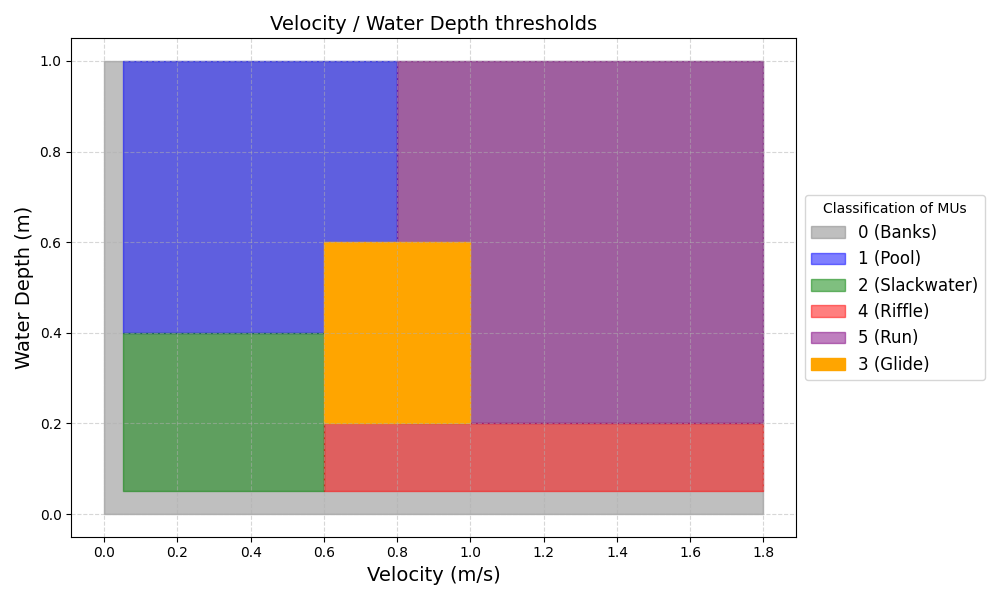
\includegraphics[width=5.5in]{images/7_MU_classification.png}
	\caption{Velocity and water depth thresholds.}
	\label{fig:MU_thresholds}
\end{figure}

\begin{figure}[!htbp]
	\centering
	\includegraphics[width=5.5in]{images/3_MU+measurement.png}
	\caption{Morphological units classification and calibration-validation data sets.}
	\label{fig:MU}
\end{figure}

\subsection{Bayesian calibration using Gaussian Process Regression for single and multiple calibration targets}\label{sec:sec2.6}

\subsubsection{Bayesian Inference using metamodels}
\label{subsec:sec2.6.1}
Calibration reduces the discrepancy between model outputs and observed data by modifying sensitive input parameters. Bayesian principles support this process by accounting for sources of uncertainty in the calibration parameters \( \omega = \{\omega_1, \omega_2, \ldots, \omega_N\} \) using  prior probability functions and measured data  \(D_P\) through a likelihood function. This results in an updated probabilistic knowledge of the uncertain parameters called posterior distribution function \cite{smith1992bayesian,lim2017comprehensive}. Bayes` Theorem is represented as: 

\[
P(\omega | D_P) = \frac{P(D_P | \omega) \cdot P(\omega)}{P(D_P)}
\]

where \( P(\omega | D_P) \) is the posterior distribution function of the uncertain model parameters given measured data \(D_P\), \(P(D_P | \omega)\)  is the likelihood function,  \( P(\omega) \) is the prior probability function, which  shows the prior knowledge of the uncertain parameters and finally \( P(D_P) \) is the so called marginal likelihood which serves as a normalization constant.  

Applying Bayesian principles using Monte Carlo or Markov-Chain Monte Carlo in real computationally expensive models is time-consuming or simply unfeasible \cite{smith1992bayesian,oladyshkin2020bayesian3}.
Thus, the development of machine learning algorithms that approximate complex models while maintaining their accuracy has been the focus of recent studies in many engineering fields. For instance, in hydraulic modeling, the employment of surrogate models \( \mathcal{M}(\omega) \) also called metamodels have been getting attention to reduce computational cost in multiparametric and highly complex simulations and perform stochastic analysis in light of measured data.

The current study approximates the complex hydromorphodynamic model \( M_c \) using Gaussian Process Emulators (GPE) also called GP metamodels \( \mathcal{M}(\omega) \). A metamodel approximates the complex model response \( M_c \) (e.g. hydromorphodynamic outputs) using data-driven function approximation approaches \cite{razavi2012review} employing only a few initial model realizations or training points. For this purpose, we run 25 initial complex model runs using Sobol sampling method as it provides uniform and efficient coverage of the parameter space \(\Omega\) \cite{garud2017design}.

With a fast-performing metamodel, we conduct Bayesian inference using Monte Carlo sampling (MC = 22000) to infer updated probability distributions of \(N = 9\) sensitive and uncertain model parameters (see Table .~\ref{tab:roughness_zones}) through rejection sampling \cite{beckers2020bayesian}. To quantify the compatibility between model outputs and measured data for each MC sample, the likelihood function plays a fundamental role, as it expresses how well the model explains the observed data. In this approach, we account for imperfections in both the modeling approaches (i.e., complex and surrogate models) and the measurements by considering a lump sum of uncertainties, combining measurement error, complex model error, and the additional error introduced by the surrogate model approximation following a Gaussian distribution. The likelihood function of the observed data given a Monte Carlo realization \( \omega_{\text{MC}} \) is:

\[
P(\bm{D} \mid \omega_{\text{MC}}) = \mathcal{N}(\bm{D} \mid \mathcal{M}(\omega_{\text{MC}}), \bm{R})
\]

where \( \bm{D} \) is the vector of observed data at \(P\) measurement locations, \( \omega_{\text{MC}} \) is one Monte Carlo realization of the parameter vector, \( \mathcal{M}(\omega_{\text{MC}}) \) is a vector containing the surrogate model predictions at \(P\) measurement locations and \( \bm{R} \in \mathbb{R}^{P \times P} \) is the total covariance matrix over all measurement locations as 
\[
\mathbf{R} = \sum_{p=1}^{P} \left( \mathbf{\Sigma}_{\text{complex}} + \mathbf{\Sigma}_{\text{surrogate}} + \mathbf{\Sigma}_{\text{measurement},p} \right)
\]

Note that if the likelihood function incorporates more than one variable, it becomes a multivariate likelihood. In this study, when using the MOGP metamodel the likelihood employs the two surrogate model outputs from the multioutput metamodel (i.e., water depth and velocity) to compute a multivariate likelihood , doubling the size of the necessary vectors and matrices for likelihood computation. The expanded likelihood function becomes: 

\[
P(\bm{D} \mid \omega_{\text{MC}}) = \frac{1}{\sqrt{(2\pi)^P |\bm{R}|}} \exp\left( -\frac{1}{2} \left( \bm{D} - \mathcal{M}(\omega_{\text{MC}}) \right)^\top \bm{R}^{-1} \left( \bm{D} - \mathcal{M}(\omega_{\text{MC}}) \right) \right)
\]

where \( \bm{D} - \mathcal{M}(\omega_{\text{MC}}) \) is the residual vector, representing the difference between the measured data and the model output evaluated at each Monte Carlo sample \( \omega_{\text{MC}} \). A resulting likelihood vector will contain the likelihood values of all the MC parameter combinations, from which some will be filtered out through rejection sampling \cite{smith1992bayesian} to obtain a posterior (post-calibration) distribution of the calibration parameters \(\omega\). Furthermore, a maximum a posteriori set of parameters can be extracted from the post-calibration distributions and conceived as the parameter set that best approaches the measured data.


\subsubsection{Single output and Multi output Gaussian Process Emulators}
\label{subsec:sec2.6.2}

A metamodel using Gaussian Process Regression \( \mathcal{M}(\omega) \) is employed to approximate a complex hydromorphodynamic model \( M_c (\omega) \) and perform Bayesian model calibration and uncertainty quantification of the selected calibration parameters \(\omega\). The approach centers primarily in the estimation of two model outputs that share underlying dependencies such as velocity and water depth. At each  measurement location, both variables are computed by the complex model and extracted to create 25 input-output sets for the initial metamodel training. Typically, one can predict each output of interest separately by training single output Gaussian Process (SOGP) metamodels denoted as:

\[
M_c^{(t)}(\omega) \approx \mathcal{M}^{(t)}(\omega) \approx \mathcal{GP}(\mu^{(t)}(\omega), k(\omega, \omega'))
\]

where \( \mathcal{M}^{(t)}(\omega) \) is a single-output Gaussian Process metamodel trained specifically for output type \( t \) and measurement location \( x,y \)  (i.e., velocity or water depth) with input parameters \( \omega \).  \( \mu^{(t,x,y)}(\omega) \) is the mean function defining the expected value of the surrogate model, and \( k(\omega, \omega') \) is the covariance function or kernel, which defines the dependencies between function values at different input locations \( \omega \) and \( \omega' \). 

In general, an advantage of Gaussian Processes is their ability to provide not only predictions of output quantities but also their associated uncertainties \cite{lindholm2022machine}, making them suitable for various engineering applications such as Bayesian calibration and uncertainty quantification of expensive and multi-parametric models. For instance, \citeA{schwindt2023bayesian} and \citeA{mouris2023stability} have implemented Gaussian Process Emulators to simplify complex reservoir models and perform stochastic calibration. However, in many real-world cases, some variables are correlated and may contain valuable information that can be shared among them to improve the learning process of any metamodel by exploiting their correlations \cite{breiman1997predicting}. The application of multitask learning in hydro-morphodynamic modeling has not yet been explored and could undoubtedly be leveraged for calibration purposes. The fundamental concept of multitask learning is the sharing of knowledge acquired from several tasks while they are simultaneously trained \cite{caruana1997multitask}. Modeling outputs in isolation may lead to the loss of this information, potentially increasing the amount of training data required for accurate surrogate modeling or diminishing accuracy in the surrogate for a fixed amount of training sets \cite{liu2018remarks}.

To predict the two correlated variables simultaneouly (i.e., tasks) and exploit their existing correlations we use a Multioutput (or Multitask) Gaussian Process (MOGP) approach with \textbf{GPyTorch} \cite{gardner2018gpytorch}. Our case involves an isotopic and symetric Multioutput Gaussian Process (MOGP) in which the model learns all outputs from the same training sets and all outputs (i.e., water depth and velocity) have the same training importance \cite{liu2018remarks}. As described in \citeA{bonilla2007multitask}, a key difference with a SOGP is the inclusion of a task covariance matrix \( K_{lk}^{f} \), which is defined through a kernel function \( k^{f}{(t_l, t_k)} \) over task-descriptor features \( t \) to model dependencies across tasks. This kernel is then combined with a standard kernel over the input space \(k(\omega, \omega')\) to define a joint covariance function that captures both input-dependent and inter-task correlations. In the context of our study, a task descriptor \( t \) refers to the physical nature of each output (e.g., meaning two tasks which corresponds to scalar velocity or water depth at a given location), allowing the model to recognize and exploit relationships between outputs based on their physical meaning. The joint kernel function is represented by: 

\[
 k_{\text{MO}}\big((\omega, l), (\omega', k)\big) =  K_{lk}^{f} \cdot k(\omega, \omega')
\]

where, \( k_{\text{MO}}\big((\omega, l), (\omega', k)\big) \) is the multioutput kernel, \( k(\omega, \omega') \) is a standard covariance function over the input parameters \( \omega \), and  \( K_{lk}^{f} = k^{f}{(t_l, t_k)} \) is a task kernel.

To represent the approximation of the complex model for two tasks \( l \) and \( k \), the multioutput Gaussian Process (MOGP) can be written as:

\[
M_c^{(l,k,x,y)}(\omega) \approx \mathcal{M}^{(l,k,x,y)}(\omega) \approx \mathcal{GP}\left(\mu^{(l,k,x,y)}(\omega),\ k_{\text{MO}}\left((\omega, l), (\omega', k)\right)\right)
\]
where \( \mathcal{M}^{(l,k)}(\omega) \) is the multioutput surrogate model (MOGP) for output types \( l \) and \( k \) given the input parameter vector \( \omega \).


For the MOGP case, the task kernel \( k^{f}{(t_l, t_k)} \) is internally computed by the Gaussian Process framework, meaning the user only provides the input parameter covariance function \( k(\omega, \omega') \), a rank for inter-tasks correlations and the number of tasks. For the SOGP, only an input parameter covariance function is provided. In both cases, a Matérn covariance function is assigned. A spetial highlight is done for SOGP because besides the calibration process using MOGP, we provide a comparison of uncertainty evolution over training data size for single and multioutput Gaussian Process. It is worth noting that, to ensure a fair comparison, both surrogate approaches are evaluated under identical conditions, including the same input kernel functions, number of iterations and learning rates.


\subsubsection{Iterative Bayesian Updating of the GP Surrogate Models}
\label{subsec:sec2.6.3}
An optimal selection of training points has a significant impact on the accuracy of GPEs \cite{sinsbeck2017sequential}. To address this, active learning strategies for Gaussian Process (GP) models optimize the selection of the most informative data points for training, thereby improving predictive accuracy with fewer training samples. Due to the complexity of acquiring informative training points in computationally demanding models, \citeA{oladyshkin2019connection} suggests a useful strategy in which relevant regions in the parameter space \(\Omega\) for surrogate training are adaptively identified by connecting Bayesian Inference with information theory. The current work uses a Bayesian Active Learning approach (BAL) as described in \citeA{oladyshkin2020bayesian3} to iteratively add new training points to the GP model. In each BAL iteration, the surrogate model is re-trained with a newly selected, more informative training point. This point is chosen from an exploration set of \texttt{mc\_exploration}~$= 2000$ samples drawn from the original prior pool of MC samples \texttt{MC}~$= 22000$. BAL selects the most informative sample (i.e., parameter combination) that led to the highest Relative Entropy (RE) or Bayesian Model Evidence (BME) during an exploitation phase involving \texttt{mc\_exploitation}~$= 1000$ evaluations. BME indicates the quality of the model against the available data while RE quantifies the information gained by comparing the prior and posterior distributions of the calibration parameters. Since evaluating BME and RE directly from the complex hydromorphodynamic model \( M_c \), we approximate BME and RE from the GP metamodel \( \mathcal{M} \) as:

\[
\text{BME}_{\mathcal{M}} \equiv p_{\omega}(\mathbf{D}|\mathcal{M}) \approx \text{BME}_{M_c} \equiv p_{\omega}(\mathbf{D}|M_c)
\]

\[
\text{DKL}\left[ p(\omega \mid \mathbf{D}, \mathcal{M}) \,\|\, p(\omega \mid \mathcal{M}) \right] \approx \text{DKL}\left[ p(\omega \mid \mathbf{D}, M_c) \,\|\, p(\omega \mid M_c) \right]
\]

\citeA{oladyshkin2020bayesian3} suggests that a stopping criterion for BAL iterations is reached when the surrogate model response $\mathcal{M}$ converges toward the complex model response $M_c$ meaning Relative Entropy (RE) and Bayesian Model Evidence (BME) also converge and stabilize over a plateau when plotted against the number of BAL iterations. For the purpose of the current work, 75 BAL iterations were required to reach a plateau durinh the MOGP training. 

%For \( MC \) Monte Carlo samples (or realizations), the matricial representation of the surrogate model outputs for velocity \( \mathbf{V} \) and water depth \( \mathbf{H} \) or a combination of both variables \( \mathbf{VH} \) and at P measurement locations is:
%
%\[
%\mathbf{V} = \begin{pmatrix}
%	v_{11} & v_{12} & \dots & v_{1P} \\
%	v_{21} & v_{22} & \dots & v_{2P} \\
%	\vdots & \vdots & \ddots & \vdots \\
%	v_{MC1} & v_{MC2} & \dots & v_{MCP}
%\end{pmatrix}
%\]
%
%\[
%\mathbf{H} = \begin{pmatrix}
%	h_{11} & h_{12} & \dots & h_{1P} \\
%	h_{21} & h_{22} & \dots & h_{2P} \\
%	\vdots & \vdots & \ddots & \vdots \\
%	h_{MC1} & h_{MC2} & \dots & h_{MCP}
%\end{pmatrix}
%\]
%
%\[
%\mathbf{VH} = \begin{pmatrix}
%	v_{11} & h_{11} & v_{12} & h_{12} & \dots & v_{1P} & h_{1P} \\
%	v_{21} & h_{21} & v_{22} & h_{22} & \dots & v_{2P} & h_{2P} \\
%	\vdots & \vdots & \vdots & \vdots & \ddots & \vdots & \vdots \\
%	v_{MC1} & h_{MC1} & v_{MC2} & h_{MC2} & \dots & v_{MCP} & h_{MCP}
%\end{pmatrix}
%\]
%
%

\subsection{Stochastic Bayesian calibration framework}
{\label{sec:Sec2.7}} 

The calibration approach uses scalar velocities and water depths collected at 37 measurement points. Relied on an initial model run and hydrodynamic outputs for pre- and post-flush conditions at the base flow, we delineated morphological units and instream roughness zones to subdivide the riverbed into spatially varying roughness patches, as shown in Fig \ref{fig:MU}. 

The surrogate-assisted calibration framework starts with the selection of nine sensitive model parameters: eigth roughness zones and the Critical Shields parameter for the first sediment class represented by a vector \( \omega \) formingthe parater space \(\Omega\) (See Table \ref{tab:roughness_zones})

\begin{equation}
	\omega = \left\{
	\begin{split}
		&\theta_{cr,10},\ K_{\text{pool}},\ K_{\text{slackwater}},\ K_{\text{glide}}, \\
		&K_{\text{riffle}},\ K_{\text{run}},\ K_{\text{backwater}},\ K_{\text{wake}},\ K_{\text{LW}}
	\end{split}
	\right\}
\end{equation}


%Among all the considered roughness zones, five correspond to morphological units such as pool, slackwater, glides, riffles, and runs covering the entire main river bed. Additionally, backwater, wake and LW specific regions are taken into account. 

To facilitate the comparison between different metamodel approaches, we conducted Bayesian calibration of the model utilizing both Single-Output Gaussian Processes (SOGP) and a Multi-Output GP (MOGP).

The calibration framework proceeds as follows:

\textbf{First}, we performed 25 initial complex model runs. These training points are common for training three initial GP metamodels (SOGP -scalar velocity, SOGP -water depth and MOGP -water depth \& scalar velocity). The surrogates are trained at each measurement location where data for calibration is available.

\textbf{Second}, we fixed 75 BAL iterations, adequate for RE and BME stabilization. Upon completion of the BAL iterations, we quantified model parameter uncertainty via Bayesian inference using the last trained SOGP and MOGP metamodels,  to obtain posterior distributions of the calibration parameters. This allows us to quantify uncertainty of the selected model parameters and verify which metamodel approach provides high probability regions that potentially fit better the measured data. 

\textbf{Third}, we select the 'best performing' set of parameters as the maximum a posteriori (MAP) estimate from the posterior distributions after Bayesian inference. To test the effectiveness of the proposed calibration methodology, the best-performing set of parameters is evaluated using both the complex model and the MOGP model. The results are then compared to those of a base model that assumes a uniform Nikuradse roughness coefficient \(K_{NKU_{UN}}\) along the entire riverbed. 

The study uses the Root Mean Squared Error (RMSE) as the statistical metric for comparing measured data and complex/surrogate model outputs. Specifically, one RMSE value is reported for each calibration quantity (velocity and water depth), computed as the mean error over all 37 measurement points. RMSE is calculated using both the complex model and the surrogate model outputs, allowing a direct comparison of their predictive accuracy against measured data.

\begin{equation}
	\text{RMSE} = \sqrt{ \frac{1}{P} \sum_{i=1}^{P} (T_i - \hat{t}_i)^2 }
\end{equation}

where \( P \) is the number of measurement points (\( P = 37 \)), \( T_i \) is the measured value at point \( i \), and \( \hat{t}_i \) is the model-predicted value at point \( i \), either from the complex model or the surrogate model.


%We believe that current stochastic calibration methodology may efficiently identify the ideal roughness values across morphological units and roughness zones, supporting the thorough investigation of roughness combinations that best match the measured data.

\subsection{Assessment SOGP and MOGP performance}
\label{sec:sec2.8}
The study assesses the evolution of the Root Mean Squared Error (RMSE), the Pearson correlation coefficient (\(r\)), and the mean width of the confidence intervals (CI) during a metamodel validation step, depending on the increase in training points for both Single-Output (SO) and Multi-Output (MO) Gaussian Process metamodels. For this purpose, we used 25 randomized parameter sets to test the prediction of the two variables after every 5 BAL iterations. The effectiveness of BAL is investigated with training set sizes ranging from 25 to 100 points, to further evaluate whether the surrogates' accuracy improves as the training set size increases.

\section{Results}

\subsection{GP metamodel assessment over training points iterations}

This assessment evaluates the evolution of the GP metamodels over increasing numbers of training points. It is tested using three statistical metrics: Root Mean Squared Error (RMSE), the Pearson correlation coefficient (\(r\)), and the mean width of the confidence intervals (CI) to approximate two hydromorphodynamic quantities in a metamodel validation stage. 

\subsubsection{Water Depth}
Figure~\ref{fig:your_figure_label}~(a) shows the evolution of three metrics for the approximation of water depth. The RMSE for the MOGP starts relatively high compared to the SOGP and fluctuates until it stabilizes at approximately 0.11\,m after the 30\textsuperscript{th} training iteration. In contrast, the SOGP slightly improves its RMSE over time and reaches about 0.12\,m by the 100\textsuperscript{th} iteration.
Regarding the correlation coefficient, MOGP improves as more training data is added, reaching values between 0.86 and 0.88 after the 50\textsuperscript{th} training point. In comparison, the SOGP reaches its highest correlation value (approximately 0.86) at the 100\textsuperscript{th} training step. This trend suggests that \textbf{BAL} contributes to improving the surrogate’s performance after the 30\textsuperscript{th} training point for both cases.

The evolution of the mean width of the confidence intervals (CI) for SOGP exhibits a more consistent behavior as the number of training points increases. In contrast, the MOGP shows greater fluctuations during the early stages but gradually narrows the CI width over time, converging to values similar to those of the SOGP.

\subsubsection{Scalar Velocity}
Similarly to water depth, Figure~\ref{...}b) shows the evolution of three metric quantities for the approximation of scalar velocity. The RMSE for MOGP exhibits a fluctuating behavior similar to that observed for water depth during the early stages of training, eventually stabilizing after the 60\textsuperscript{th} iteration at a value of 0.085, compared to 0.095 for SOGP. In the case of SOGP, the RMSE slightly increases but follows a more stable trend. The correlation index for MOGP outperforms SOGP by reaching values over 0.89, compared to SOGP which attains a maximum of 0.86 at the 100\textsuperscript{th} iteration. Regarding the mean confidence interval (CI) width, MOGP shows a lower value (approximately 0.15), while SOGP shows a slight increase as training points are added, reaching 0.25.

\begin{figure}[!htbp]
	\centering
	\begin{minipage}[b]{0.49\textwidth}
		\centering
		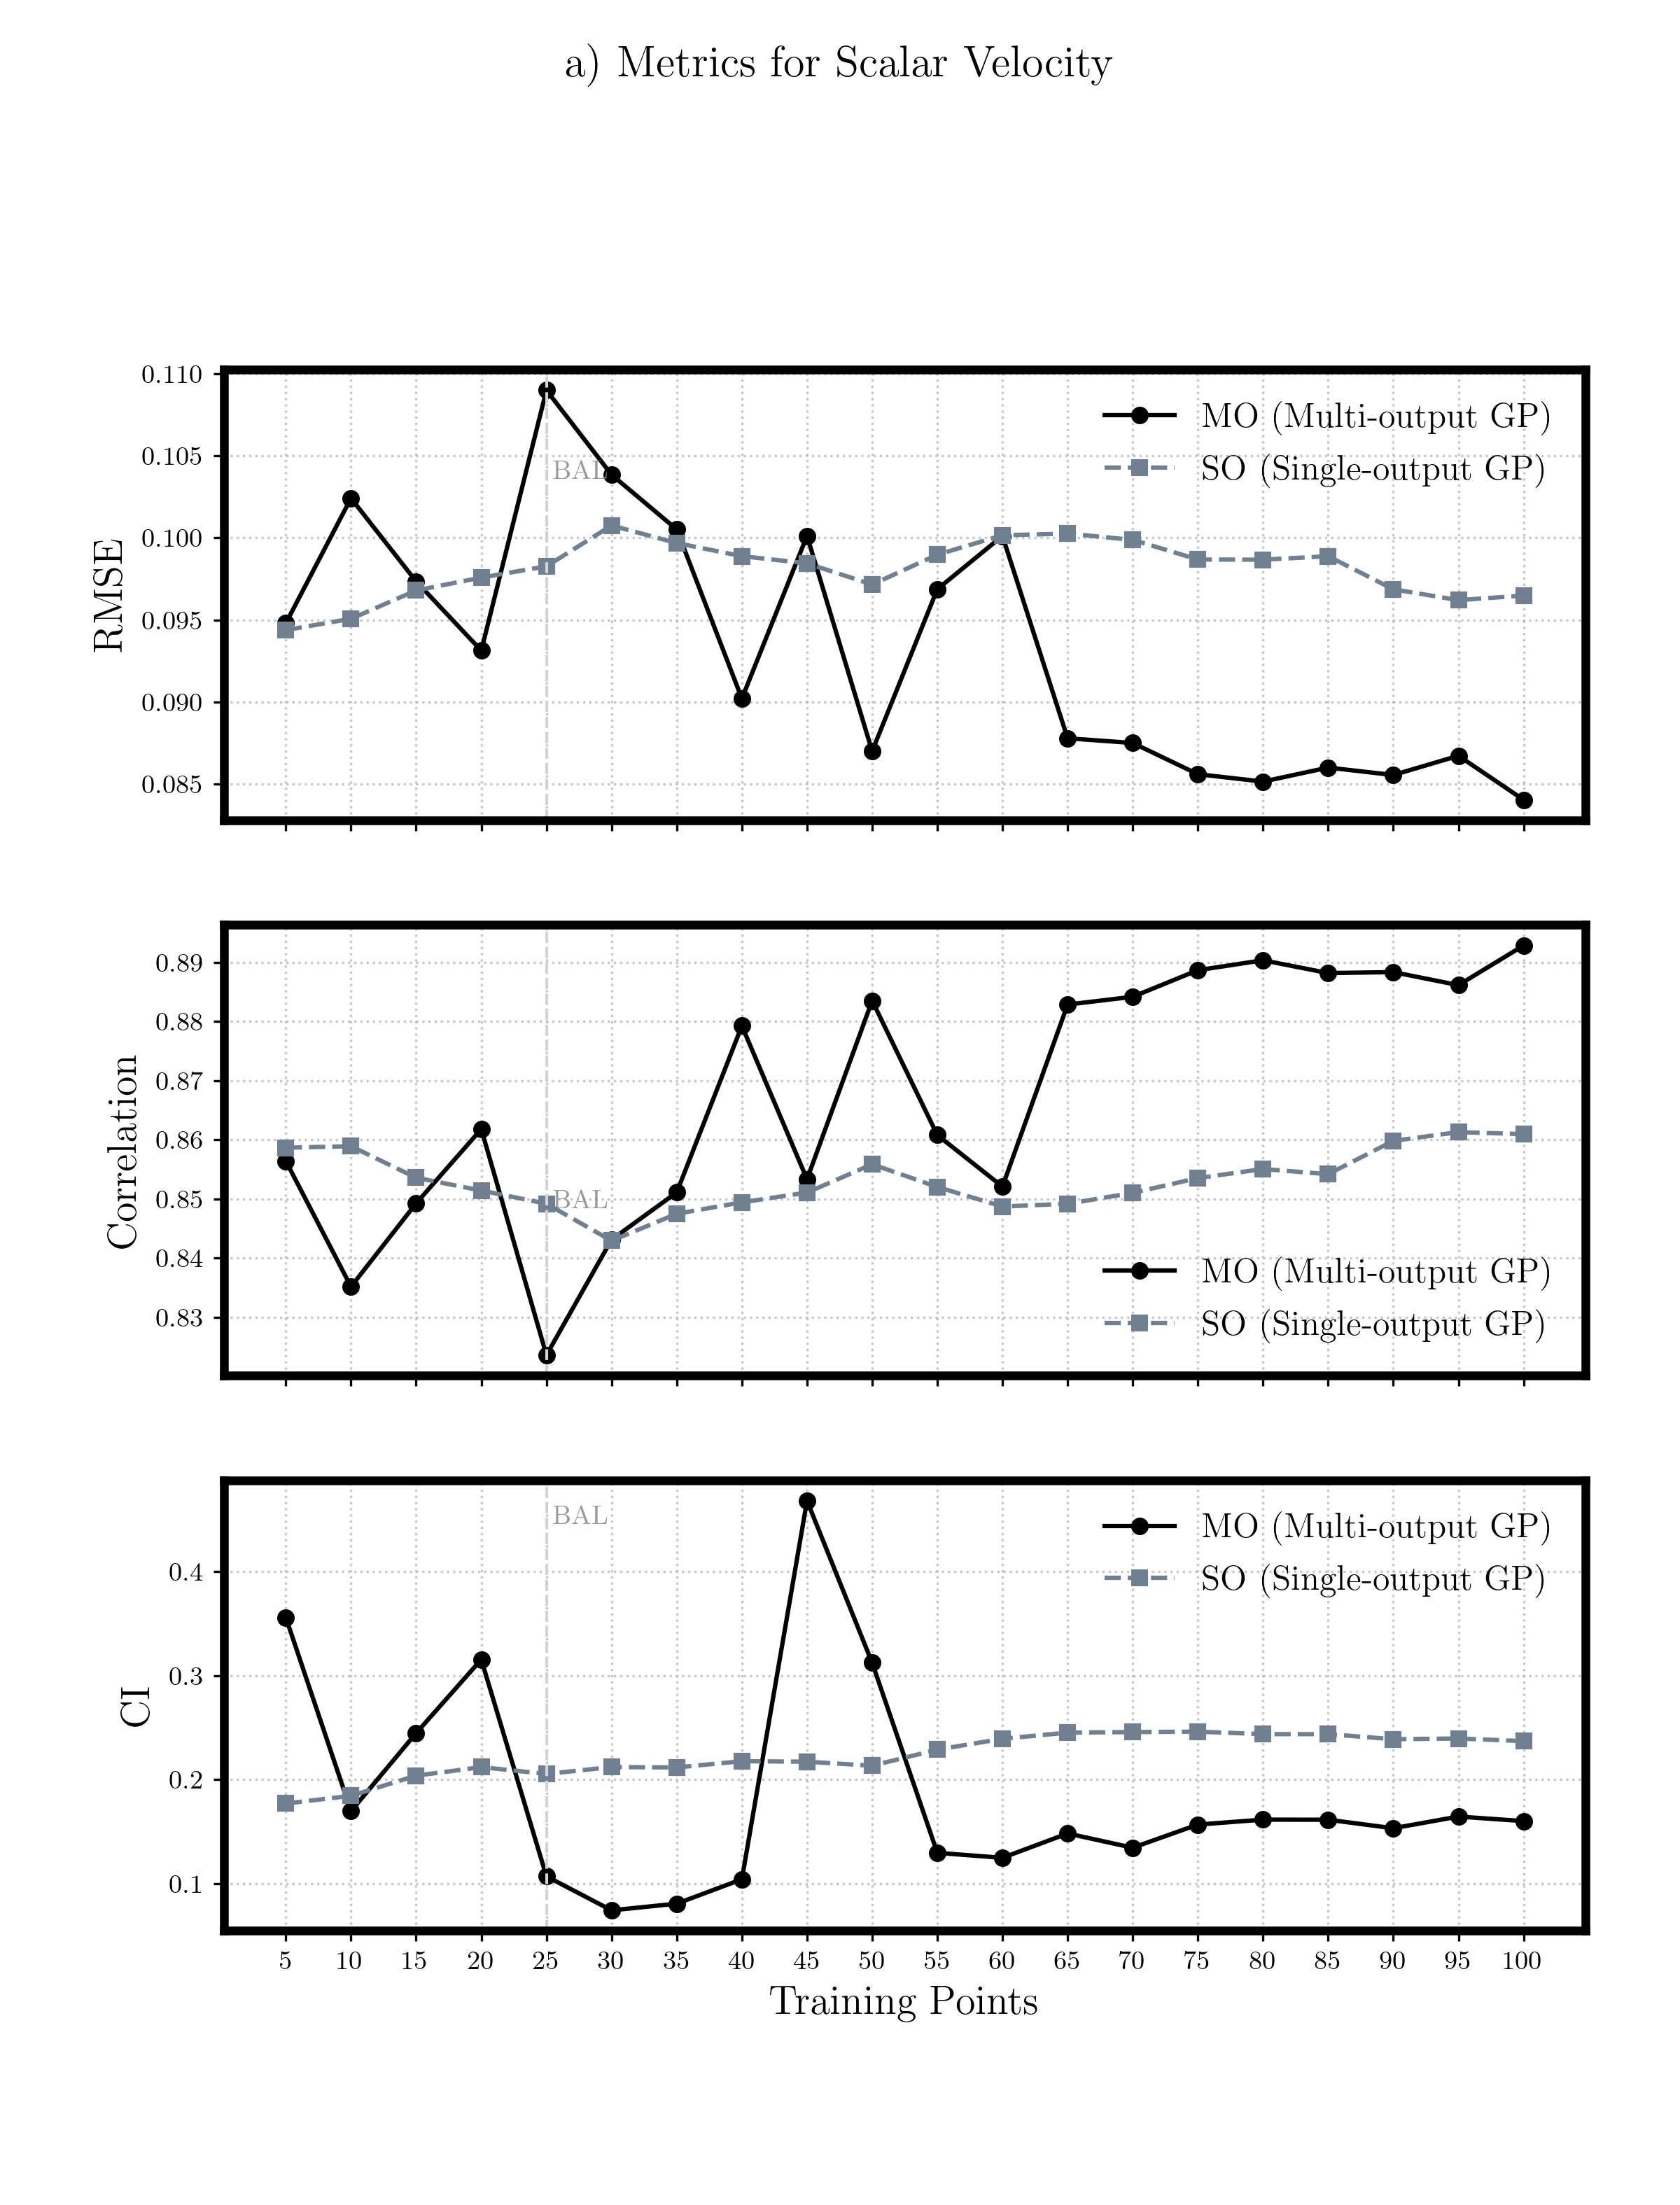
\includegraphics[width=\textwidth]{images/8a_meta-validation-SV.png}
		\caption{(a) Metamodel validation results for scalar velocity.}
		\label{fig:meta_validation_sv}
	\end{minipage}
	\hfill
	\begin{minipage}[b]{0.49\textwidth}
		\centering
		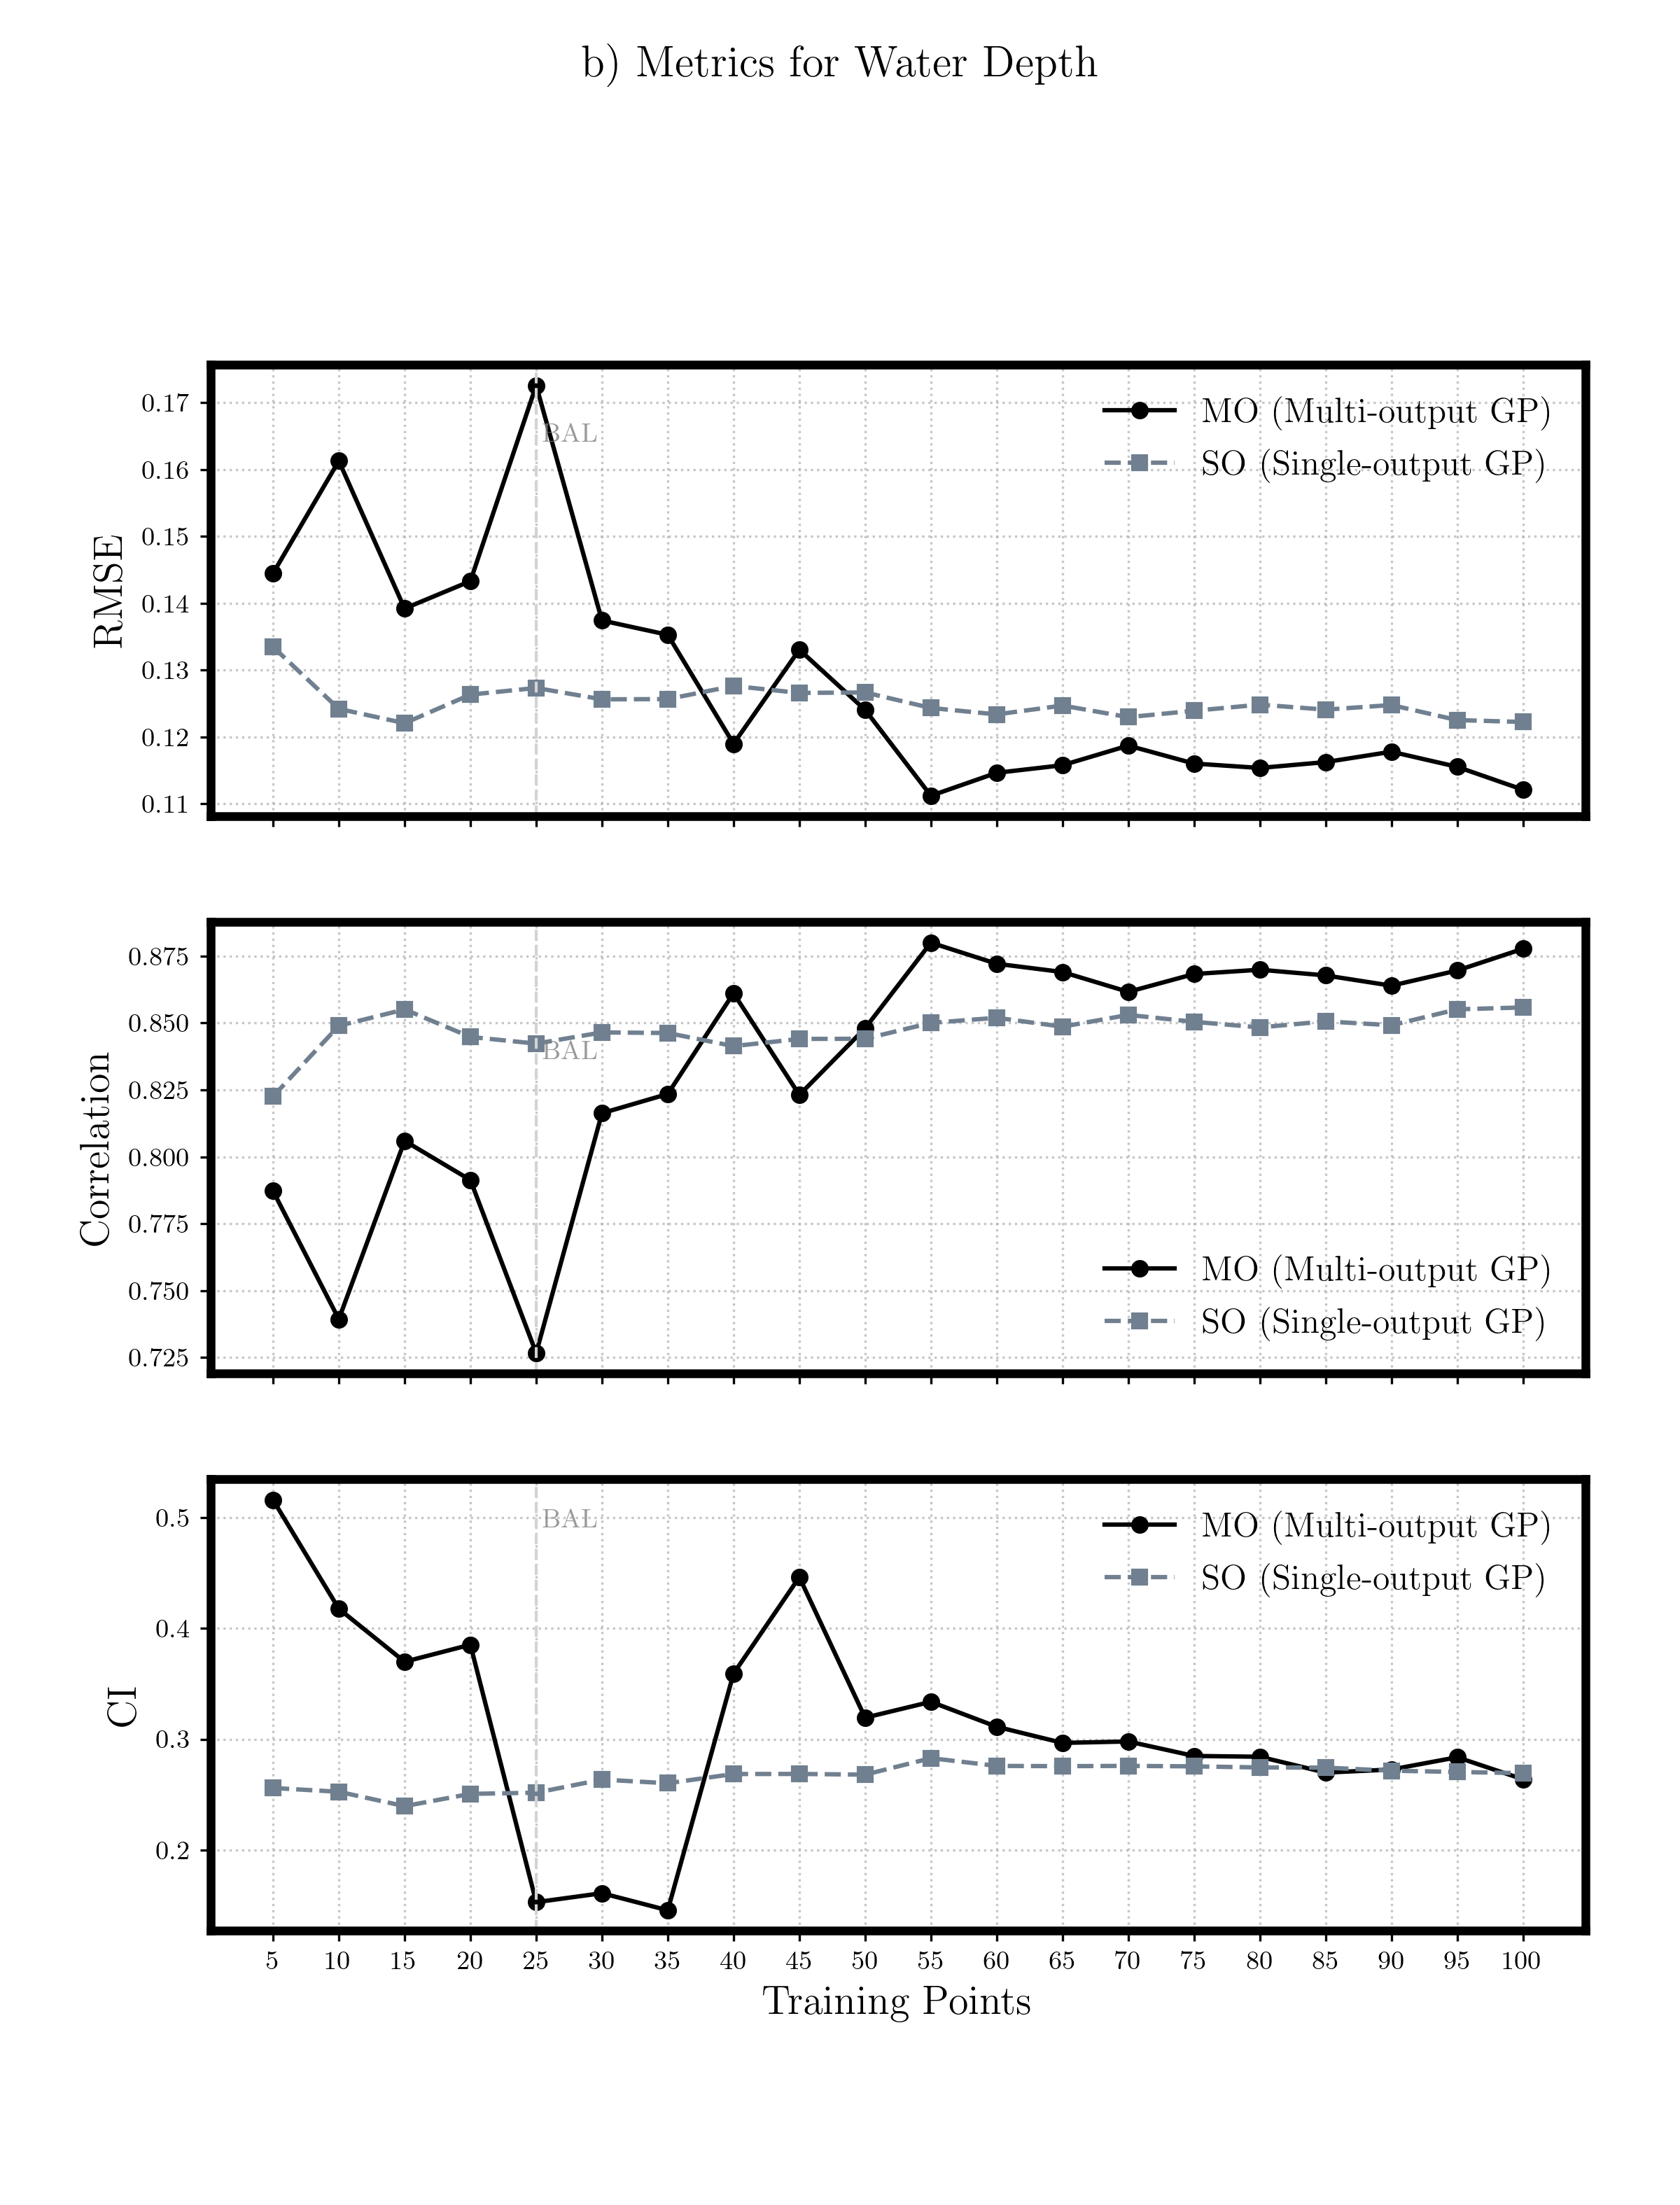
\includegraphics[width=\textwidth]{images/8b_meta-validation-WD.png}
		\caption{(b) Metamodel validation results for water depth.}
		\label{fig:meta_validation_wd}
	\end{minipage}
\end{figure}

\subsection{Convergence speed of the metamodel}


\subsection{Uncertainty quantification of calibration parameters}

Each model realization needed approximately 17 minutes and each Bayesian Inference - BAL iteration took on average 4 minutes. The posterior distributions after Bayesian Inference represent the updated probability of the calibration model parameters after measured data was included in the analysis.

\textbf{Critical Shields Parameter}

The posterior distribution for the Critical Shields Parameter shows an skewness toward higher values, showing a clear peak near 0.069. The analysed Critical Shields parameter correspond to the first class, suggesting a dominant bedload transport during peak flow events with high shear stresses  on fine sediments, thus the Bayesian Inference compensates by favoring higher values of Critical Shields parameter. 

\textbf{Pools}
The posterior distribution of the Nikuradse coefficient in Pool indicate a moderate higher probability at the middle values, centering around 0.33~m. Initially, our prior assumption took in consideration roughner zones, so this behaviopur may suggest that the model requires slightly rougher substrate in pools to match hydrodynamic needs.

\textbf{Slackwater}
From the posterio distribution of slackwater it can be seen that the parameter keeps its uncertain behavior and lacks dominant mode. This may be attributed to a lack of suffiecient measurement points in low velocity and water depth zones.

\textbf{Glide}
The posterior distribution of glides show a higher probability region at around cenetered values with moderate spread. From the results can be seen that these roughness regions demand similar textural characteristics to keep hydrodynamic patterns at a post flush condition. The value of Nikuradse coefficient that showed a higher probability region for this roughness zone is 0.27.

\textbf{Riffles}

High probability region for Nikuradse roughess coefficient at riffles are located at low values rounding 0.125~m. This may indicate that these areas demand smoother substrate after a flush event.

\textbf{Runs}

A high probability region can be seen around 0.52~m. This suggestes that runs maintain a coarse texture even after flushing, possibly due to sustained high shear stress conditions that prevent sediment deposition and keeping its rougher surface. 

\textbf{Backwater, Wake and LW} \\

The posterior distributions for backwater areas reflect a slight skewness toward low values around 0.09. This may indicate that after a flush event, that area may require a smoother surface to reach hydrodynamic values. Similarly, the distribution for Wake is relatively narrow and centered around 0.3 m, suggesting a consistent roughness regime in wake regions. However, since no clear higher probability can be seen, this may suggest the need for denser measurements to better constrain these parameters. Finally, the distribution for LW (Large Wood) zones concentrates around values of 0.34 m. This indicates a highly uncertain behavior of the parameter in regions where the degree of certainty in the roughness estimate for these hypothetical zones is low, highlighting their sensitivity in hydrodynamic calibration, even in the absence of extensive measurements.

\begin{figure}[htbp]
	\centering
	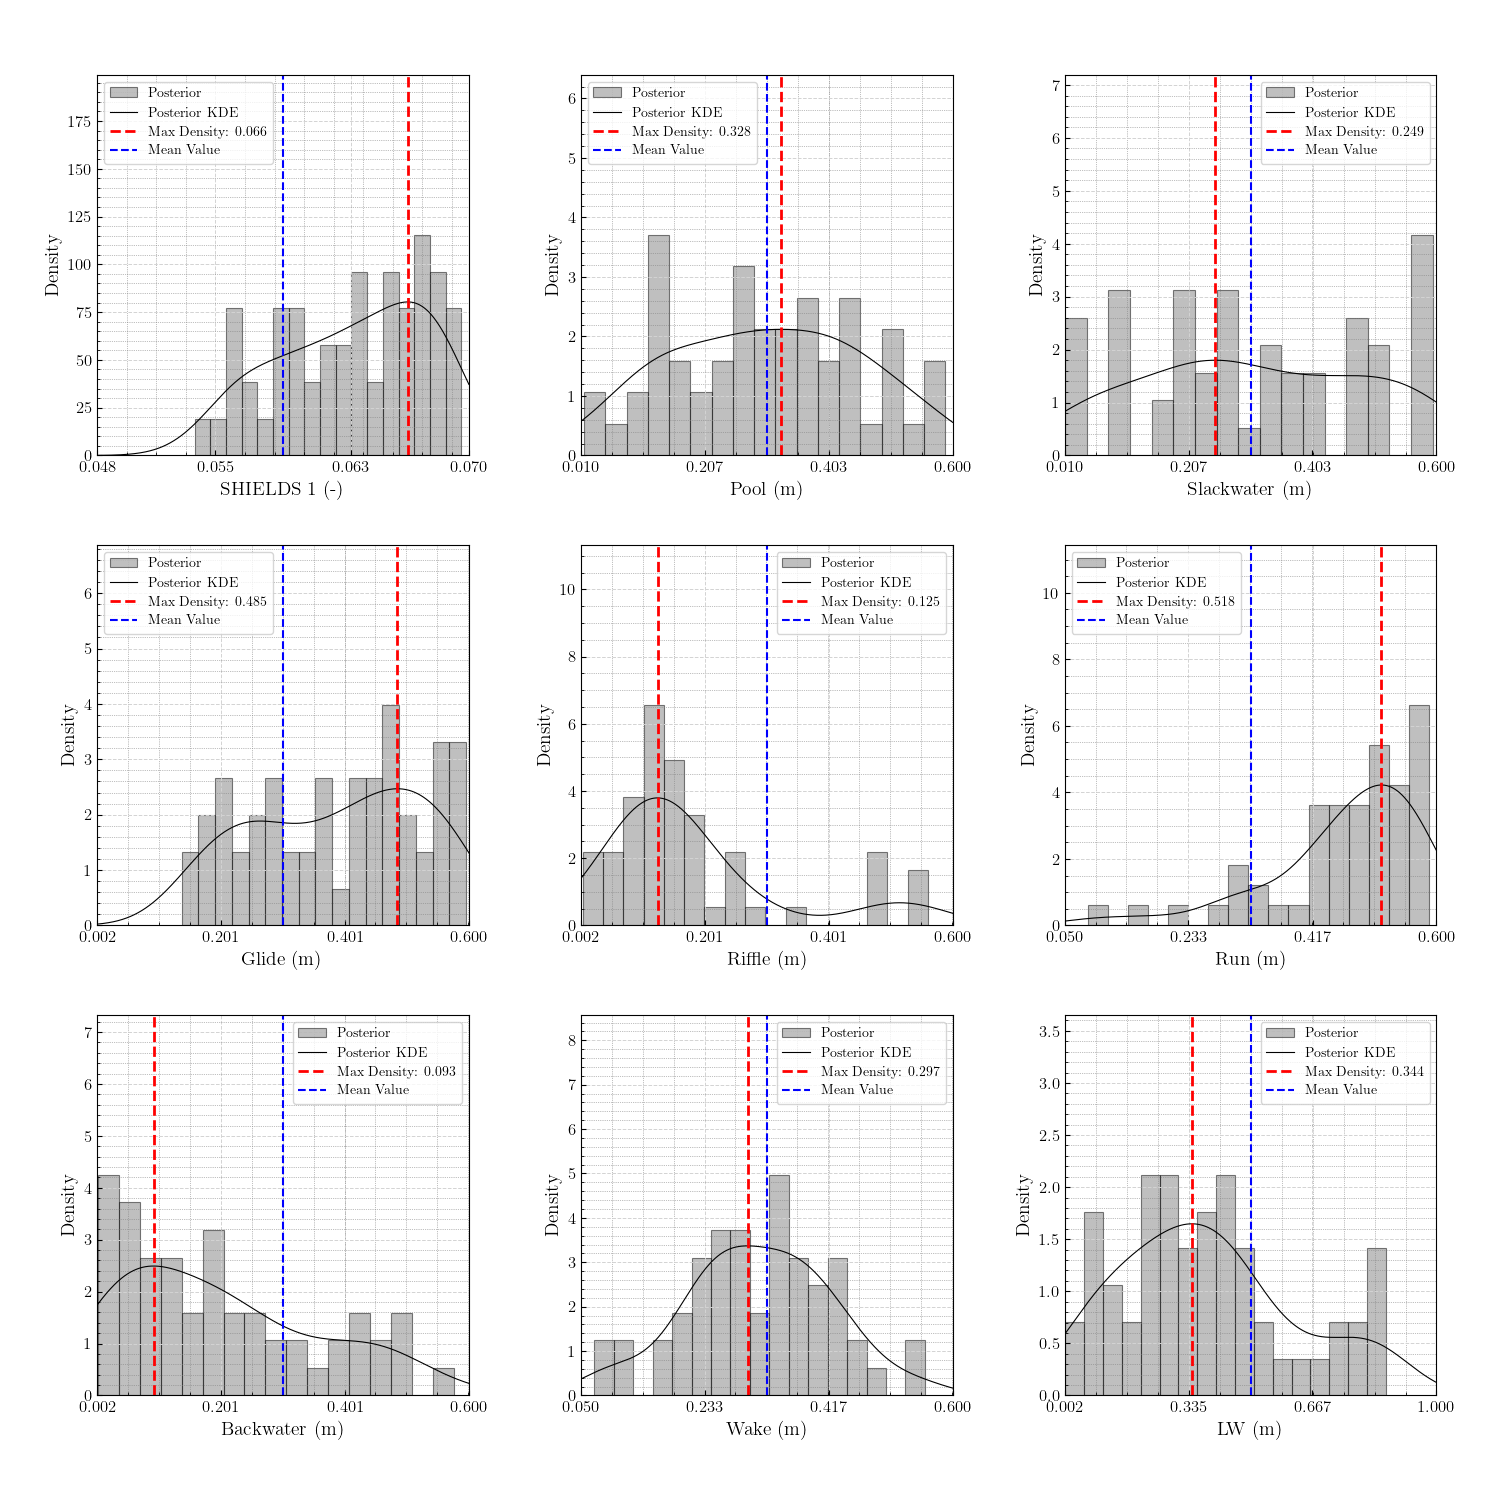
\includegraphics[width=1\textwidth]{images/posterior_distributions_iteration_76-WD-SV.png}
	\caption{Posterior distributions of model parameters using MOGP.}
	\label{fig:posterior_distributions}
\end{figure}

\subsubsection{Lump-sum calibration statistics}



% --- END OF RESULTS ACCORDING TO THE TEST PROCEDURE SECTION ---

\section{Discussion}





%%%%%%%%%%%%%%%%%%%%%%%%%%%%%%%%%%%%%%%%%%%%%%%%%%%%%%%%%%%%%%%%
%
%  ACKNOWLEDGMENTS
%
% The acknowledgments must list:
%
% >>>>	A statement that indicates to the reader where the data
% 	supporting the conclusions can be obtained (for example, in the
% 	references, tables, supporting information, and other databases).
%
% 	All funding sources related to this work from all authors
%
% 	Any real or perceived financial conflicts of interests for any
%	author
%
% 	Other affiliations for any author that may be perceived as
% 	having a conflict of interest with respect to the results of this
% 	paper.



\acknowledgments


%% ------------------------------------------------------------------------ %%
%% References and Citations

%%%%%%%%%%%%%%%%%%%%%%%%%%%%%%%%%%%%%%%%%%%%%%%
%
% \bibliography{<name of your .bib file>} don't specify the file extension
%
% don't specify bibliographystyle
%%%%%%%%%%%%%%%%%%%%%%%%%%%%%%%%%%%%%%%%%%%%%%%

\bibliography{hydro-informatics}



%Reference citation instructions and examples:
%
% Please use ONLY \cite and \citeA for reference citations.
% \cite for parenthetical references
% ...as shown in recent studies (Simpson et al., 2019)
% \citeA for in-text citations
% ...Simpson et al. (2019) have shown...
%
%
%...as shown by \citeA{jskilby}.
%...as shown by \citeA{lewin76}, \citeA{carson86}, \citeA{bartoldy02}, and \citeA{rinaldi03}.
%...has been shown \cite{jskilbye}.
%...has been shown \cite{lewin76,carson86,bartoldy02,rinaldi03}.
%... \cite <i.e.>[]{lewin76,carson86,bartoldy02,rinaldi03}.
%...has been shown by \cite <e.g.,>[and others]{lewin76}.
%
% apacite uses < > for prenotes and [ ] for postnotes
% DO NOT use other cite commands (e.g., \citet, \citep, \citeyear, \nocite, \citealp, etc.).
%

\end{document}



%More Information and Advice:

%% ------------------------------------------------------------------------ %%
%
%  SECTION HEADS
%
%% ------------------------------------------------------------------------ %%

% Capitalize the first letter of each word (except for
% prepositions, conjunctions, and articles that are
% three or fewer letters).

% AGU follows standard outline style; therefore, there cannot be a section 1 without
% a section 2, or a section 2.3.1 without a section 2.3.2.
% Please make sure your section numbers are balanced.
% ---------------
% Level 1 head
%
% Use the \section{} command to identify level 1 heads;
% type the appropriate head wording between the curly
% brackets, as shown below.
%
%An example:
%\section{Level 1 Head: Introduction}
%
% ---------------
% Level 2 head
%
% Use the \subsection{} command to identify level 2 heads.
%An example:
%\subsection{Level 2 Head}
%
% ---------------
% Level 3 head
%
% Use the \subsubsection{} command to identify level 3 heads
%An example:
%\subsubsection{Level 3 Head}
%
%---------------
% Level 4 head
%
% Use the \subsubsubsection{} command to identify level 3 heads
% An example:
%\subsubsubsection{Level 4 Head} An example.
%
%% ------------------------------------------------------------------------ %%
%
%  IN-TEXT LISTS
%
%% ------------------------------------------------------------------------ %%
%
% Do not use bulleted lists; enumerated lists are okay.
% \begin{enumerate}
% \item
% \item
% \item
% \end{enumerate}
%
%% ------------------------------------------------------------------------ %%
%
%  EQUATIONS
%
%% ------------------------------------------------------------------------ %%

% Single-line equations are centered.
% Equation arrays will appear left-aligned.

% Math coded inside display math mode \[ ...\]
%  will not be numbered, e.g.,:
%  \[ x^2=y^2 + z^2\]

%  Math coded inside \begin{equation} and \end{equation} will
%  be automatically numbered, e.g.,:
%  \begin{equation}
%  x^2=y^2 + z^2
%  \end{equation}


% % To create multiline equations, use the
% % \begin{eqnarray} and \end{eqnarray} environment
% % as demonstrated below.
% \begin{eqnarray}
%   x_{1} & = & (x - x_{0}) \cos \Theta \nonumber \\
%         && + (y - y_{0}) \sin \Theta  \nonumber \\
%   y_{1} & = & -(x - x_{0}) \sin \Theta \nonumber \\
%         && + (y - y_{0}) \cos \Theta.
% \end{eqnarray}

%If you don't want an equation number, use the star form:
%\begin{eqnarray*}...\end{eqnarray*}

% Break each line at a sign of operation
% (+, -, etc.) if possible, with the sign of operation
% on the new line.

% Indent second and subsequent lines to align with
% the first character following the equal sign on the
% first line.

% Use an \hspace{} command to insert horizontal space
% into your equation if necessary. Place an appropriate
% unit of measure between the curly braces, e.g.
% \hspace{1in}; you may have to experiment to achieve
% the correct amount of space.


%% ------------------------------------------------------------------------ %%
%
%  EQUATION NUMBERING: COUNTER
%
%% ------------------------------------------------------------------------ %%

% You may change equation numbering by resetting
% the equation counter or by explicitly numbering
% an equation.

% To explicitly number an equation, type \eqnum{}
% (with the desired number between the brackets)
% after the \begin{equation} or \begin{eqnarray}
	% command.  The \eqnum{} command will affect only
	% the equation it appears with; LaTeX will number
	% any equations appearing later in the manuscript
	% according to the equation counter.
	%
	
	% If you have a multiline equation that needs only
	% one equation number, use a \nonumber command in
	% front of the double backslashes (\\) as shown in
	% the multiline equation above.
	
	% If you are using line numbers, remember to surround
	% equations with \begin{linenomath*}...\end{linenomath*}
	
	%  To add line numbers to lines in equations:
	%  \begin{linenomath*}
		%  \begin{equation}
			%  \end{equation}
		%  \end{linenomath*}
	
	
	
